\chapter{Graph Theory}

\section{Notions}

\begin{itemize}
	\item Node : Point du graphe
	\item Edge : Connection sur le graphe
	\item Path : Séquences de nœuds de tel sorte qu'il y ait une edge entre chaque paire qui existe sur le graphe
	\item Simple Path : Chemin contenant au plus une fois un même nœud
	\item Distance between two nodes : Le plus court chemin entre deux nœuds
	\item Cycle :
	\item Connected graph :
	\item Component : Sous-ensemble de nœuds tel que :
	\begin{itemize}
		\item Le sous-ensemble est \textbf{connexe}
		\item Le sous-ensemble est \textbf{maximal} ("Prend tout le graphe")
	\end{itemize}
\end{itemize}

\section{Triadic closure}

Soit 3 nœuds $A$, $B$, et $C$. Si $A$ est connecté à $B$ et $C$ est connecté à $B$, il y a de grande chances que $A$ et $C$ se connectent.

\begin{figure}[H]
    \centering
    \includegraphics[width=0.25\textwidth]{triadic_closure}
    \caption{Exemple de Triadic closure}
\end{figure}

\subsection{Strong connection}

Dans une triadic closure, si $A$ est fortement connecté à $B$ et que $C$ est aussi fortement lié à $B$, alors $A$ est faiblement lié à $C$.

\section{Clustering coefficient}

\begin{equation}
	CC(A) = \frac{Nombre de paires d'amis de A qui sont amis enter eux}{Nombre d'amis de A}
\end{equation}

\begin{figure}[H]
    \centering
    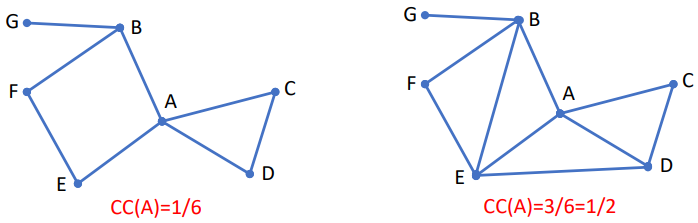
\includegraphics[width=0.4\textwidth]{clust_coef}
    \caption{Exemple de clustering coefficient}
\end{figure}

\section{Bridge}

Edge qui si retirée augmente le nombre de composants du graph.

\begin{figure}[H]
    \centering
    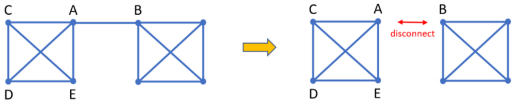
\includegraphics[width=0.4\textwidth]{bridge}
    \caption{Exemple de bridge}
\end{figure}

\subsection{Local bridge}

Edge qui si retirée la distance pour rejoindre l'autre nœud est strictement supérieure à 2.

\begin{figure}[H]
    \centering
    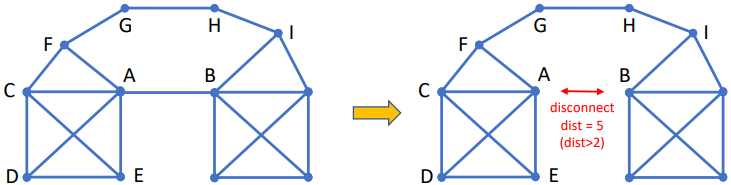
\includegraphics[width=0.4\textwidth]{local_bridge}
    \caption{Exemple de local bridge}
\end{figure}

\subsection{Neighborhood overlap}

Permet de calculer le nombre de local bridges.

\begin{equation}
overlaping(A, B) = \frac{\text{Nombre d'amis de A ET B}}{\text{Nombre d'amis de A OU B}}
\end{equation}

\begin{itemize}
	\item[$overlaping$ = 0] Local bridge
	\item[$overlaping$ tend vers 0] "Almost" local bridge
\end{itemize}

\section{Homophily}

Décrit la tendance a être amis avec des personnes ayant des choses en commun.

\subsection{Caractéristiques immutables}

Caractéristiques impossible a changer (age, groupe ethnique, sexe, etc.).

\subsection{Caractéristiques mutables}

Caractéristiques possibles a changer (occupation, croyances, couleur de cheveux; etc.).

\subsection{Mécanismes sous-jasent}

\begin{itemize}
	\item[Selection] Choisir les gens qui te ressemblent
	\item[Social Influence] Se faire influencer par les autres (par exemple aller sur un réseau social parce que tout le monde y est) 
\end{itemize}

\section{Affiliation network}

\begin{figure}[H]
    \centering
    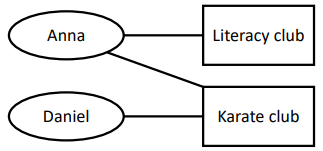
\includegraphics[width=0.25\textwidth]{affiliation_network}
    \caption{Exemple d'affiliation network}
\end{figure}

\textit{Bipartite graph} représentant les \textit{individuals} (personnes) et leurs \textit{foci} (activités).

Note : un \textit{bipartite graph} est un graphe contenant deux set de nœuds, où chaque nœud d'un set ne se connecte qu'à au moins un nœud de l'autre set.

\section{Mesurer l'homophilie}

\begin{figure}[H]
    \centering
    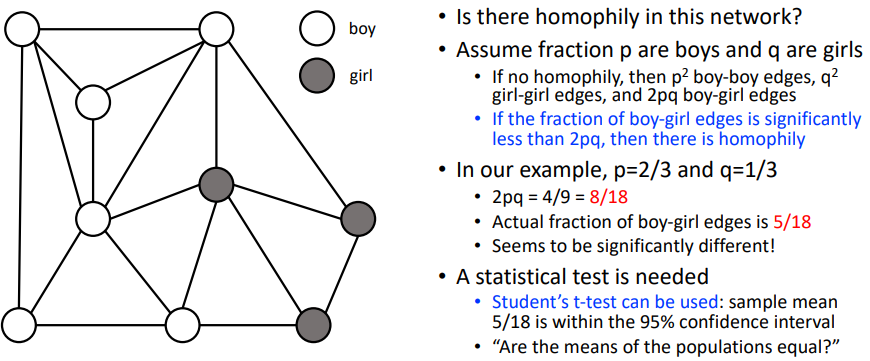
\includegraphics[width=0.25\textwidth]{homophilie_calc}
    \caption{Exemple de calcul d'homophilie}
\end{figure}

\#boys = $6$, \#girls = $3$, et \#boys-girls = $5$

Sachant que $P_b + P_g = 1$ et que $(P_b + P_g)^2 = P_b^2 + 2P_bP_g + P_g^2$\\
S'il n'y a pas d'homophilie, le nombre de liaisons boys-girls doit être $\geq$ à $2P_bP_g$\\
Ici $2P_bP_g = \frac{8}{18}$, or comme \#boys-girls = $5$ on a : $\frac{5}{18}$

Il y a donc bien de l'homophilie.

\section{Différents types de closures}

\begin{figure}[H]
    \centering
    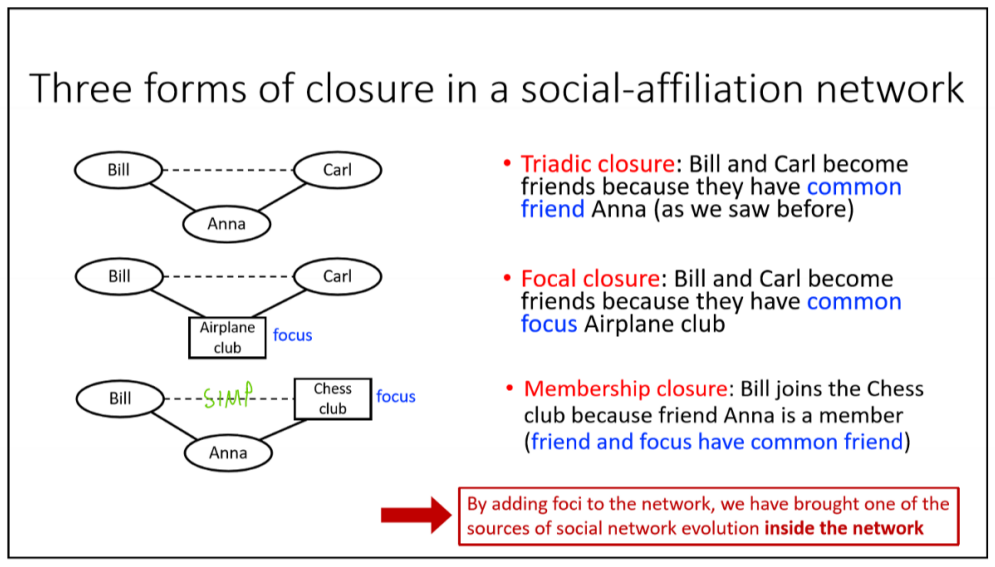
\includegraphics[width=0.7\textwidth]{closures_types}
    \caption{Différents types de closures}
\end{figure}

\section{Positive/negative relationships}

\begin{figure}[H]
    \centering
    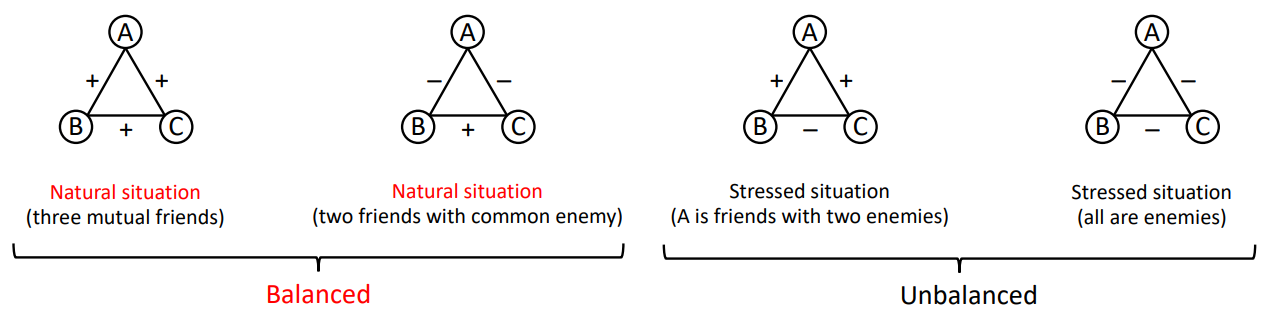
\includegraphics[width=0.8\textwidth]{structural_balance_triangles}
    \caption{Différentes configurations de triangles relationnels}
\end{figure}

\subsection{Structural balance theorem}

Si un graphe labellisé complet est équilibré, alors soit toute les paires sont amies, soit les nœuds peuvent être divisés en deux groupes tel que les nœuds au sein d'un groupe sont amis, et que les nœuds entre les groupes sont ennemis.

\paragraph{Preuve}

\begin{figure}[H]
    \centering
    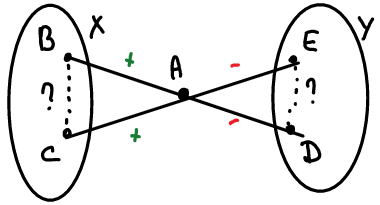
\includegraphics[width=0.2\textwidth]{structural_balance_theorem}
    %\caption{Différentes configurations de triangles relationnels}
\end{figure}

On considère qu'il y a au moins un lien négatif.\\
On définit X : A + ses amis, et Y : tout les ennemis de A.\\
On remarque facilement que B et C doivent être amis, idem pour D et E.\\
Dans ce cas :
\begin{itemize}
	\item BAC aurait une structure $++-$
	\item EDA aurait une structure $---$
\end{itemize}
Or ces structures sont exclues par la Structural Balance Hypothesis.

\chapter{Game Theory}

\section{Notions}

\begin{itemize}
	\item Payoff : Ce que rapporte un choix au joueur (profit)
	\item Strategy : Action que le joueur va faire
	\item Best response : Réaction a une action prédite d'un autre joueur
	\item Dominante strategy : La meilleure réponse à toutes les stratégies de l'autre
	\item Strictly dominante strategy : Le choix le plus avantageux peut importe l'action de l'autre joueur
\end{itemize}

\section{Hypothèses}

Pour garder des jeux équivalents, on va poser une hypothèse sur les jeux qu'on va évaluer :
\begin{itemize}
	\item Les joueurs ne comptent que sur le payoff (si le joueur est altruiste et qu'il tient compte des autres cela doit être mit dans son payoff)
	\item Tous les joueurs sont au courant de tout ce qui se passe dans le jeu
	\item Chaque joueur cherche à maximiser son profit (payoff)
\end{itemize}

\begin{table}[H]
    \centering
    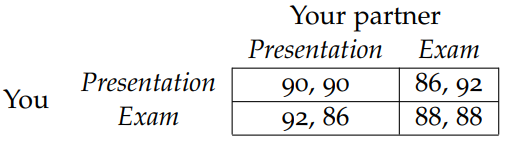
\includegraphics[width=0.4\textwidth]{choice_table}
    \caption{Exemple de tableau de choix}
\end{table}

En appliquant ces hypothèses sur l'exemple ci-dessus, on peut voir que le payoff de choisir \textit{Présentation} est de 88\% contre un payoff de 90\% si on choisit \textit{Exam}. Notre partenaire à le même choix et donc rationnellement, les deux vont choisir \textit{Exam} pour maximiser leur payoff. Cependant, on arrive dans une situation où les deux ont 88\% au lieu d'avoir 90\% 'qui est possible). C'est ce qu'on appelle un équilibre de Nash.

\section{Exemple d'équilibres}

\subsection{Formalisation : Best response}

\begin{table}[H]
    \centering
    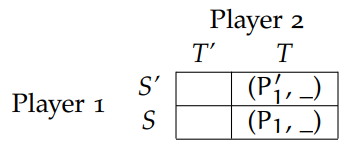
\includegraphics[width=0.25\textwidth]{best_response}
    \caption{Best response pour Player 1 si $P_1 > P1'$\\Strictly best response pour Player 1 si $P_1 \geq P'_1$}
\end{table}


\subsection{Stratégie dominante}

\begin{table}[H]
    \centering
    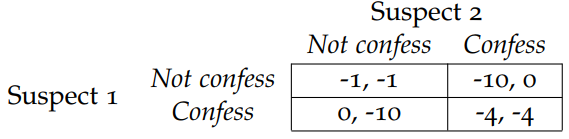
\includegraphics[width=0.4\textwidth]{dominant_strategy}
    \caption{Stratégie dominante (les deux choisissent de confesser)}
\end{table}

\subsection{Stratégie strictement dominante}

\begin{table}[H]
    \centering
    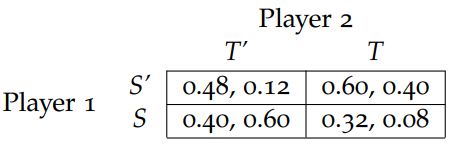
\includegraphics[width=0.35\textwidth]{strictly_dominant_strategy}
    \caption{– Stratégie strictement dominante pour Player 1 (il choisira toujours S’)}
\end{table}

\subsection{Équilibre de Nash}

Un équilibre de Nash est pour une stratégie où chaque joueurs a la meilleur réponse par rapport aux autres.

\begin{table}[H]
    \centering
    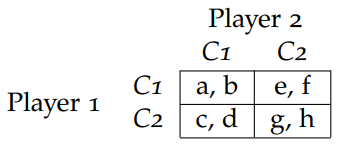
\includegraphics[width=0.28\textwidth]{nash_equilibrium}
    \caption{$P(C2, C1)$ est un équilibre de Nash si $a < c$ et $h < d$}
\end{table}

\subsection{Formalisation}

\begin{table}[H]
    \centering
    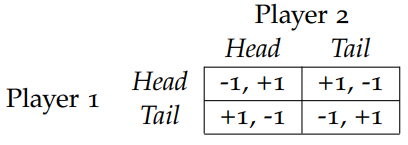
\includegraphics[width=0.35\textwidth]{mixed_strategies}
    \caption{Mixed strategy (aucun équilibre de Nash)}
\end{table}

On pose $p$ la probabilité de \textit{Player 1} de faire la stratégie \textit{Head}, et $q$ celle de \textit{Player 2}.\\
\textit{Player 1} va donc analyser les choix de son adversaire : $-p + (1-p) = 2p - 1 \Leftrightarrow p = \frac{1}{2}$.\\
De même pour \textit{Player 2}, qui obtient $q = \frac{1}{2}$.

\subsubsection{Principe d'indifférence}

Si \textit{Player 2} a tendance à plus jouer \textit{Head}, alors pour gagner \textit{Player 1} aura tendance à jouer plus \textit{Tail}.

\subsection{Équilibre pareto optimal}

Équilibre où aucun acteur ne peut améliorer sa situation sans dégrader celle de l'autre.\\
Un équilibre pareto optimal n'est pas nécessairement un équilibre de Nash (et inversement).

\begin{table}[H]
    \centering
    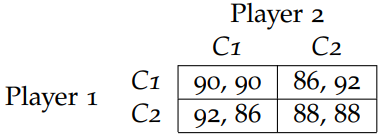
\includegraphics[width=0.3\textwidth]{nash_pareto}
    \caption{$(88, 88)$ est un équilibre de Nash tandis que les 3 autres options sont des équilibres pareto optimaux}
\end{table}

\section{Dynamic Games}

Jeux évoluant au fil de la partie.

\begin{figure}[H]
    \centering
    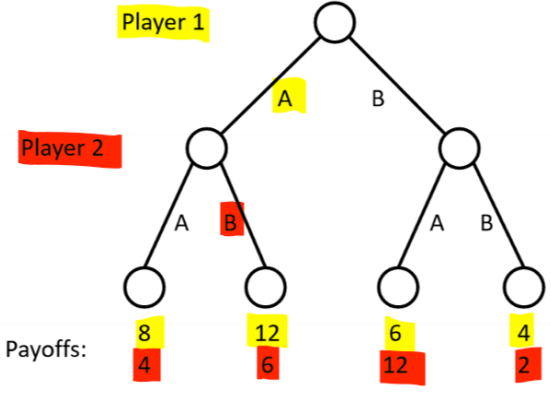
\includegraphics[width=0.3\textwidth]{dynamic_game}
    \caption{Exemple de jeu dynamique (extensive form)}
\end{figure}

\begin{table}[H]
    \centering
    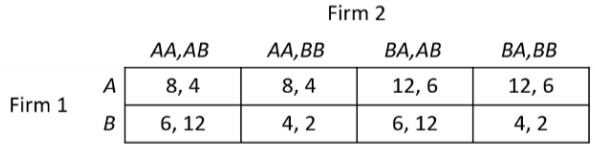
\includegraphics[width=0.5\textwidth]{dynamic_game_table}
    \caption{Exemple de jeu dynamique (normal form}
\end{table}

\section{Résumé}

\begin{figure}[H]
    \centering
    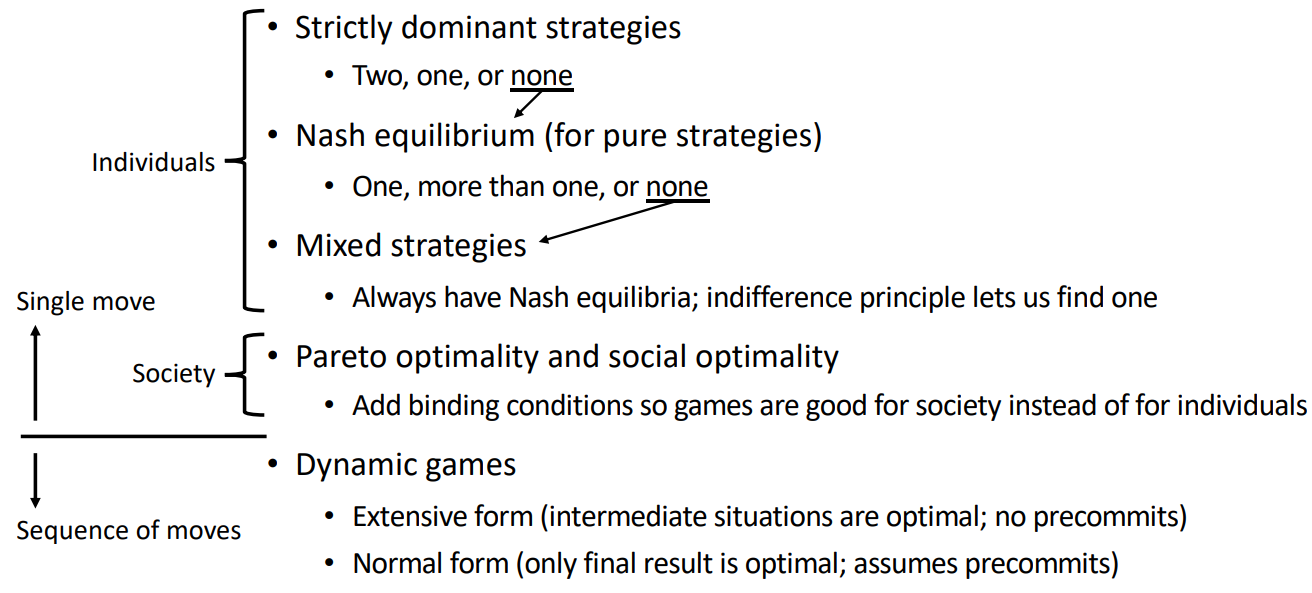
\includegraphics[width=0.8\textwidth]{game_theory_sum}
    \caption{TL;DR}
\end{figure}

